\chapter{Literature Review}

\section{Cosmic ray}


% source of cr & introduce acceleration mechanism
CRs could come from different origins from galactic
to extra-galactic sources.
% The kinetic energy of cosmic rays also 
% highly depends on where does it from.
Relatively low-energy (below a few GeVs) CRs from the Sun known as
the "solar energetic particles" are produced from the coronal mass
ejection event in which ions are dragged by a turbulent magnetic
field in the plasma.
% Low energy CRs usually came from 
% the Sun called ``solar energetic particle''. The production process of 
% solar particle event mostly came from the coronal mass ejection (CME)
% when high atomic number and energy (HZE) ions were dragged by a magnetic field in the plasma.
On the other end of the spectrum, extremely high-energy (above ~EeV)
CRs are likely from extragalactic supermassive blackholes.
The dominant Galactic sources of ~TeV CRs are hypothetically
supernova remnants (SNRs).
% The extra-galactic CRs typically 
% has high momentum from the extreme condition of the acceleration mechanism
% in pulsar, quasars and supernova remnant (SNR). 
The theoretical description of acceleration in SNR and solar flares
is the shock wave acceleration in the following paragraph.

% acceleration mechanism
One of the most impactful studies of CR's acceleration mechanism 
was conducted by \cite{fermi1949origin}. 
The study describes how high-energy CR particles gain large
momentum from the shock wave that was generated by supernovae or
violent explosions of massive stars.
% a great explosion from the heavy dense star.
This acceleration model is known as the diffusive shock acceleration
process which provides the correct description of the spectrum as
a power law in rigidity. At high-energy, the rigidity is approximately
directly proportional to the total energy ($E$).
Thus, the CR spectum can be modeled in the form
% How it gains
% the kinetic energy could be described as a first-order shock 
% acceleration and the overall spectrum of charged particles could be
% represented as the power law in Equation \ref{eq:fermi_powerlaw}.

\begin{equation}
    \frac{dN(E)}{dE} \propto E^{-\gamma}
    \label{eq:fermi_powerlaw}
\end{equation}

where $\gamma \geq 2$.
However, moving magnetized plasma cloud can accelerate the charged
particle in the space called ``second-order Fermi acceleration''.
Both regimes can be computed using the Lorentzian forces regardless of
thermal collision in the process.

% cosmic ray component paper
CR protons are major components in the arrival of CR particles
under multiple observations.
However,
$alpha$ particles (He nuclei) are the second most abundant CR
particles and should be taken into account in the calculations
of CR interactions.
% $\alpha$-particle is also 
% a second important CR particle when considering a precise calculation
% of CR interactions.
The other major nuclei in CRs
% majority of heavy weight nuclei that could propagate through space
are C, O, Ne and so on. 
Differential fluxes in kinetic energy for various nuclei from
multiple experiments are visualized in Figure \ref{fig:cr_composition}
by \cite{review_particle_physics2012}.
% The differential flux in kinetic energy of multiple observations is 
% visualized in Figure \ref{fig:cr_composition} under the work of 
% \cite{review_particle_physics2012} to take various atomic numbers 
% from various experiments.

\begin{figure}[h!]
    \centering
    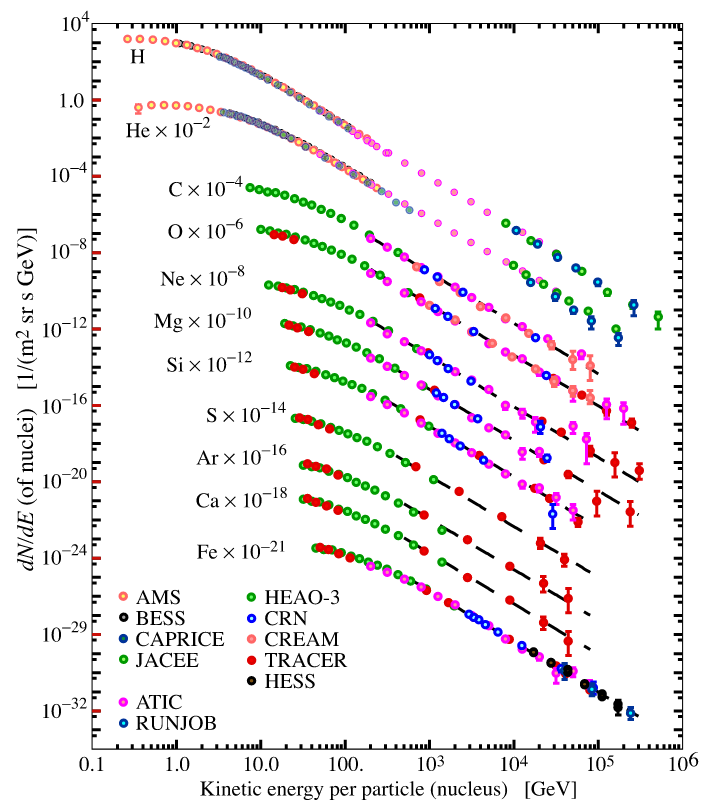
\includegraphics[width=0.6\textwidth]{content/literature_review/figures/cr_composition.png}
    \caption{CR elemental spectra from various experiments \citep{review_particle_physics2012}}
    \label{fig:cr_composition}
\end{figure}


% CR and Earth's magnetic field -> cutoff rigidity
% ctte -> cutoff rigidity
Moving plasmas inside the Earth generate the geomagnetic field
for which the north pole is at the geographical south pole of
the Earth and vice versa.
% Since there is a moving plasma inside the Earth, the magnetic field 
% has been generated from the dynamics of the moving charged ions in 
% the plasma.
% The magnetic field of the Earth has a north pole at 
% the geometric south pole of the Earth and vice versa. 
The Earth's magnetic field plays
an important role in the arrival of CR particles because the Lorentzian 
forces could bend the direction of a moving charged particle depending 
on the rigidity of the particle.
% This means the magnetic field line mantles the Earth with a
% certain direction towards the geometric north pole.

% cite -> east-west
Firstly,
the geomagnetic field creates the CR cutoff rigidity which is the
minimum rigidity of incident charged CRs to arrive at the top
of the atmosphere at different locations on Earth.
% it creates the CR cutoff rigidity on the terrestrial
% where each location of the Earth requires a minimum
% rigidity of incident charged particles as a condition for arrival. 
Figure \ref{fig:cr_map_rigidity} shows a cutoff
rigidity on the Earth's surface.

\begin{figure}[h!]
    \centering
    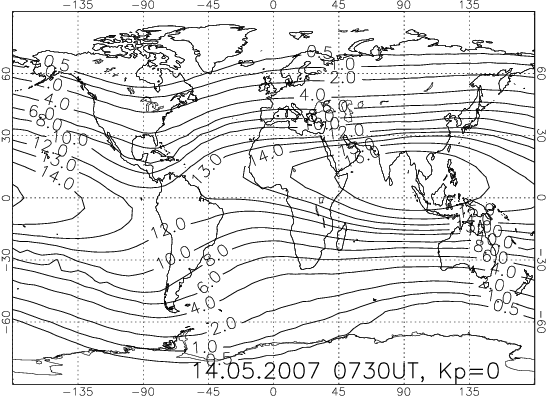
\includegraphics[width=0.6\textwidth]{content/literature_review/figures/map_cutoff_rigidity.png}
    \caption{ World map with computed geomagnetic vertical cutoff
        rigidity contour lines on a given date
        \citep*{map_cr_rigidity_cutoff}
    }
    \label{fig:cr_map_rigidity}
\end{figure}

%  east-west and Explorer XI first observe cite{kraushaar1965explorer}
Secondly,
due to the centripetal Lorentz force, charged CRs would spiral
around magnetic field lines, creating the so-called
``East-West effect" which results in the higher flux of CRs
arriving from the West than that from the East for detectors
in the low-Earth orbtis.
Historically, the detection of the East-West asymmetry of CRs
by Rossi in 1930s \citep{rossi1934} provided the first clue that
CRs are predominantly charged.
% incoming charged CRs with a charge have been dragged 
% by the Earth's magnetic. Then a charged particle would move as 
% a curve or a spiral depends on the rigidity of an incoming particle
% which leads to the East-West effects when an orbiting detector could 
% find more particle on the Westside more than on the East side for 
% a significant level of intensity.
% A pioneer of Earth's $\gamma$-ray 
% experiment is conducted by \cite{kraushaar1965explorer} where the 
% detector was deployed on the Explorer XI satellite
% and orbiting in the sky.


% east west : Kraushaar65 Kraushaar72
\begin{figure}[h!]
    \centering
        \subfloat[
            Explorer XI \citep{kraushaar1965explorer}
        ]{
            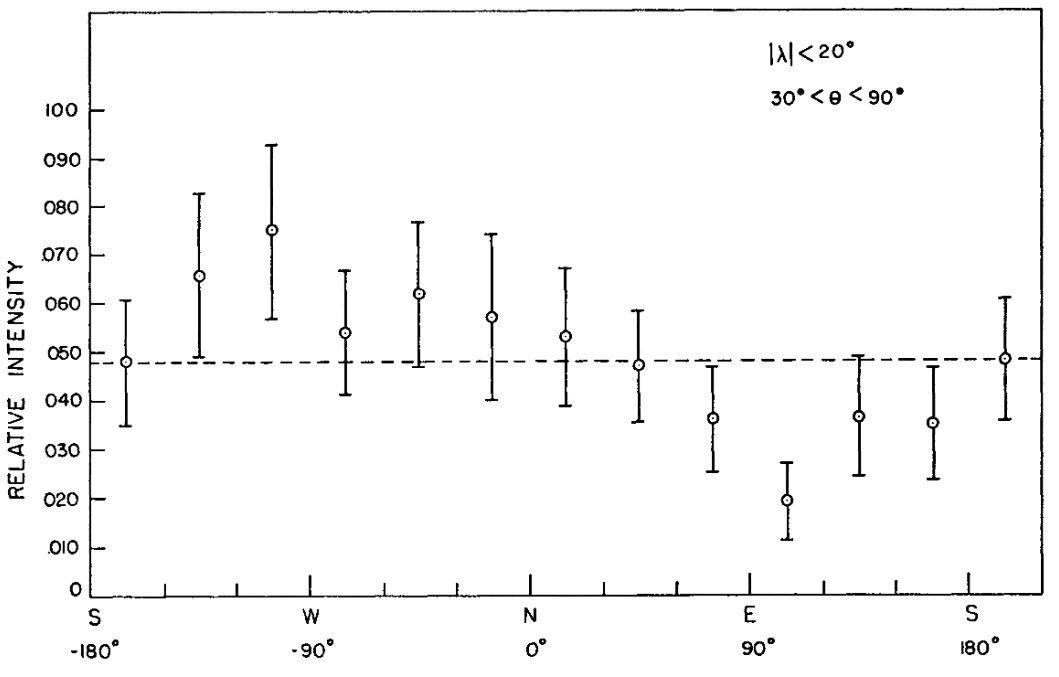
\includegraphics[width=0.48\textwidth]{content/literature_review/figures/explorer_xi_eastwest.png}
            }
        \hfill
         \subfloat[
            OSO-3 \citep{Kraushaar72}
         ]{
            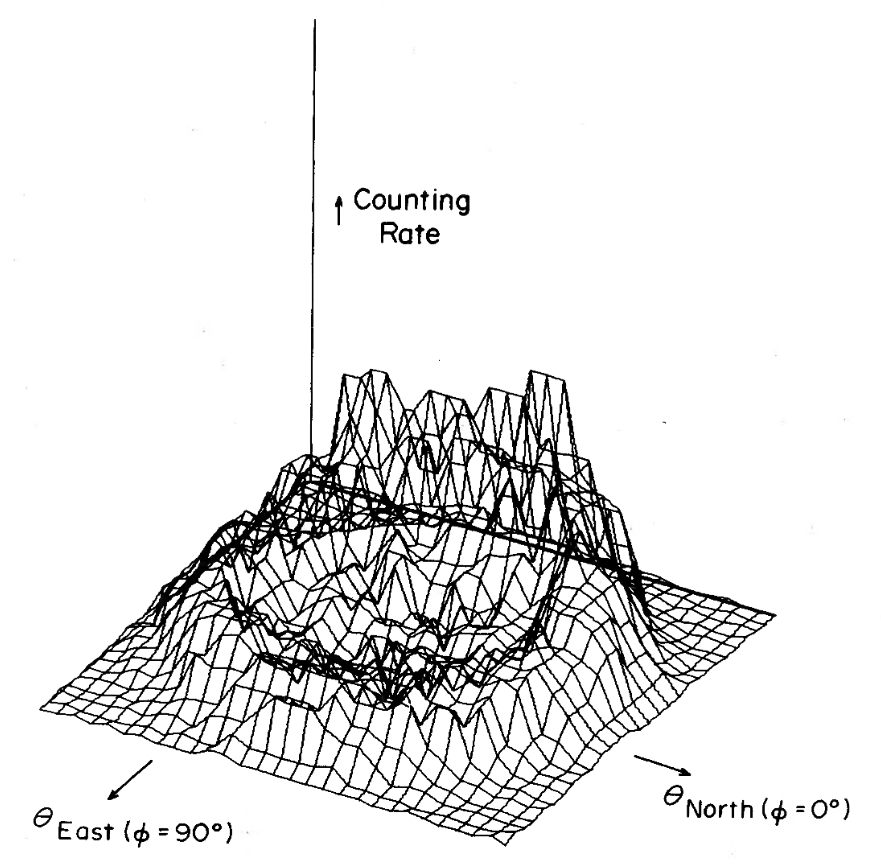
\includegraphics[width=0.48\textwidth]{content/literature_review/figures/eastwest_1972}
        }
        \caption{
            The East-West asymmetry of the Earth's $\gamma$-ray intensity
        }
       \label{fig:gamma_ew}
\end{figure}

\section{Earth's $\gamma$-ray}

When CRs interact with the Earth's upper atmosphere, hadronic
showers of secondary particles including $\pi^0$'s are produced
which then quickly decay into $\gamma$ rays.
This CR-induced $\gamma$-ray emission makes the Earth by far
the brightest $\gamma$-ray source for space-based detectors due
to the proximity. The pioneering cosmic $\gamma$-ray experiment
in space was conducted by \cite{kraushaar1965explorer} by deploying
a $\gamma$-ray detector onboard the Explorer XI satellite. 
This experiment clearly detected the Earth's $\gamma$-ray emission
and showed distinguishable intensity from the East and West as shown
in Figure \ref{fig:gamma_ew}a.
The third Orbiting Solar Observatory (OSO-3) was the second experiment 
which observed MeV-range $\gamma$ rays and studied the Earth's
emission (reference).
% The incoming photon from the East and West direction is the crucial evidence 
% of the bending of CRs trajectory by Earth's magnetosphere. The first 
% analysis shows a distinguishable intensity from East to West as visualized 
% in Figure \ref{fig:gamma_ew}a. The second experiment where
% the $\gamma$-ray detector is attached to Third Orbiting Solar
% Observatory (OSO-3) and collecting the $\gamma$-ray in MeV range.
The 2-D plot of the Earth's $\gamma$-ray intensity
is shown in Figure ~\ref{fig:gamma_ew}b.

% describe zenith
Moreover, \cite{kraushaar1965explorer} found the strong enhancement
in the $\gamma$-ray intensity in the direction near
the Earth's horizon (or limb) as shown in Figure \ref{fig:explorer_xi_zenith}a
due to CRs grazing tangentially through the Earth's upper atmosphere
and forward scattering photons towards the detector.
The observed intensity also depends on the geomagnetic
latitude location of the satellite as shown
in Figure \ref{fig:explorer_xi_zenith}b.
Since CR flux declines steeply with rigidity, low-rigidity CRs
are much more abundant than high-rigidity ones.
Therefore, the CR-induced Earth's $\gamma$-ray intensity
from high geomagnetic latitude (low cutoff rigidity) is
greater than that from the low geomagnetic latitude
as shown in Figure \ref{fig:explorer_xi_zenith}.
% Moreover, An early analysis found 
% that the observing $\gamma$-rays intensity along the zenith angle
% from different geomagnetic latitudes ($\lambda$) is differentiable
% as shown in Figure \ref{fig:explorer_xi_zenith}. The reason behind 
% this outcome came from the Earth's rigidity where the incoming 
% particles near the equatorial have less chance to arrive than the 
% north pole and likely to interact with the atmospheric molecules 
% and emits the $\gamma$-rays. This is the secondary 
% evidence of how geomagnetic fields play an important role on the 
% trajectory of the CR particles. 

\begin{figure}[h!]
    \centering
        \subfloat[
            observing above 20\textdegree geomagnetic latitude 
        ]{
            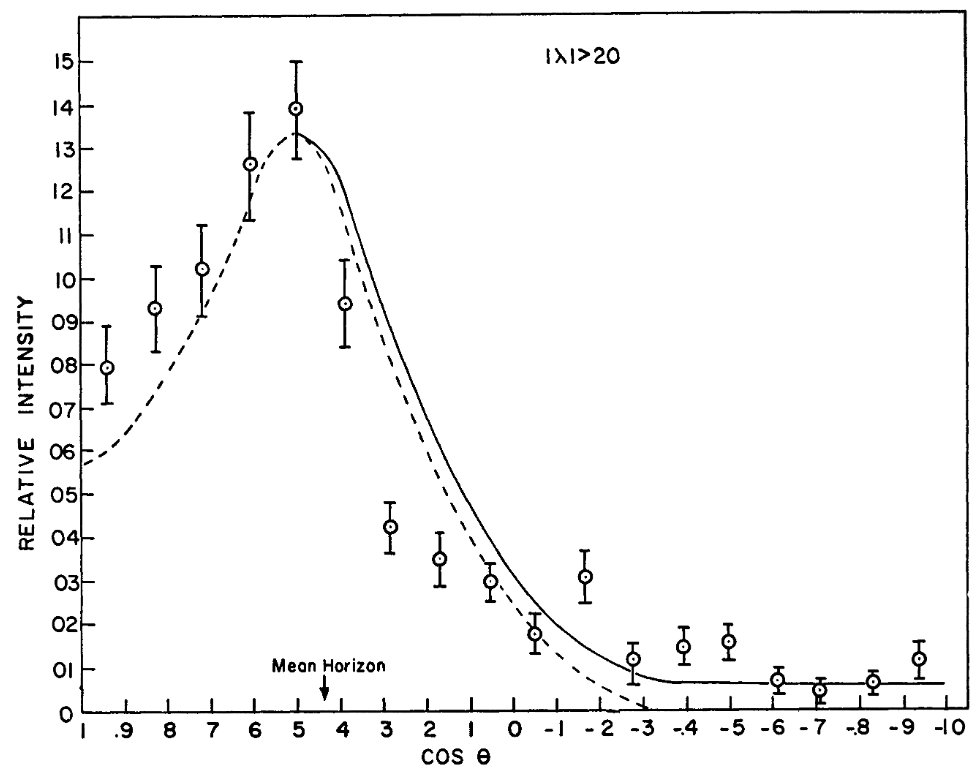
\includegraphics[width=0.48\textwidth]{content/literature_review/figures/explorer_xi_azimutal_lambda_a20.png}
            }
        \hfill
         \subfloat[
            observing below 20\textdegree geomagnetic latitude 
         ]{
            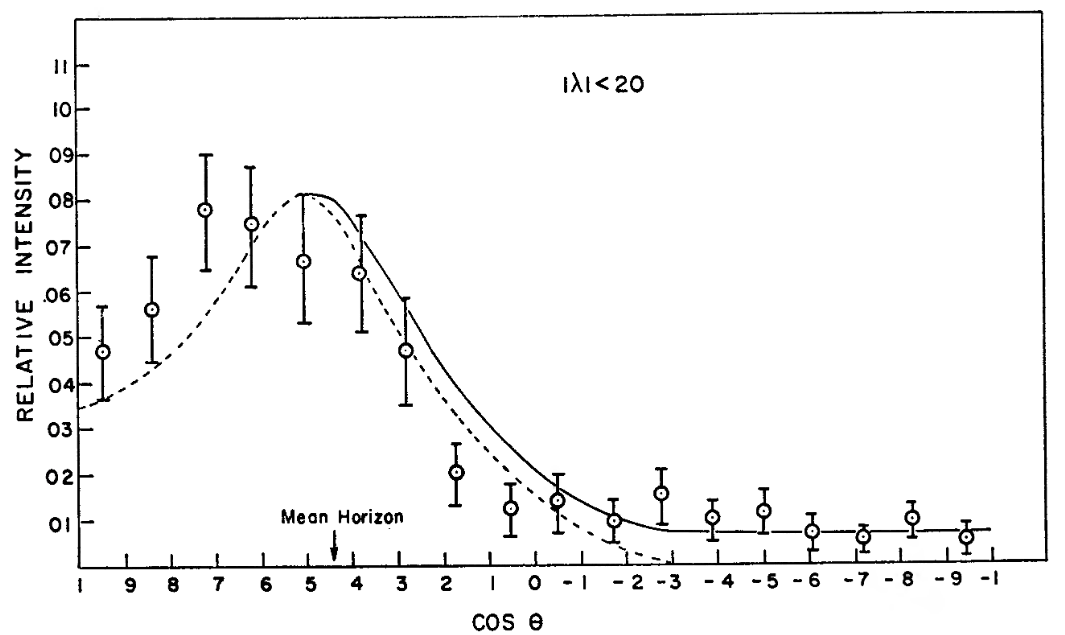
\includegraphics[width=0.48\textwidth]{content/literature_review/figures/explorer_xi_azimutal_lambda_b20.png}
        }
        \caption{
            $\gamma$-ray intensity along the zenith angle
            \citep{kraushaar1965explorer}
        }
       \label{fig:explorer_xi_zenith}
\end{figure}

% early earth gamma-ray observe -> SAS-2 (Thompson81),  EGRET (Petry05)
The following experiment of Earth's $\gamma$-ray observations was conducted 
by sending the second small astronomy satellite (SAS-2) with
a higher angular resolution at energy
% a higher resolution in angle and observing
above 35 MeV up to GeV range
\citep{Thompson81}. The projected 3-D representation of intensity
is shown in Figure \ref{fig:gamma_earth_second_wave}a. A few decades 
later, another precise $\gamma$-ray detector has been attached to the 
Compton Gamma Ray Observatory (CGRO) satellite \citep{Petry05}
which observed
% An outcome from the analysis illustrated
the bright region around the Earth's limb region as 
in Figure \ref{fig:gamma_earth_second_wave}b.


\begin{figure}[h!]
    \centering
        \subfloat[
            SAS-2 experiment \citep{Thompson81}
        ]{
            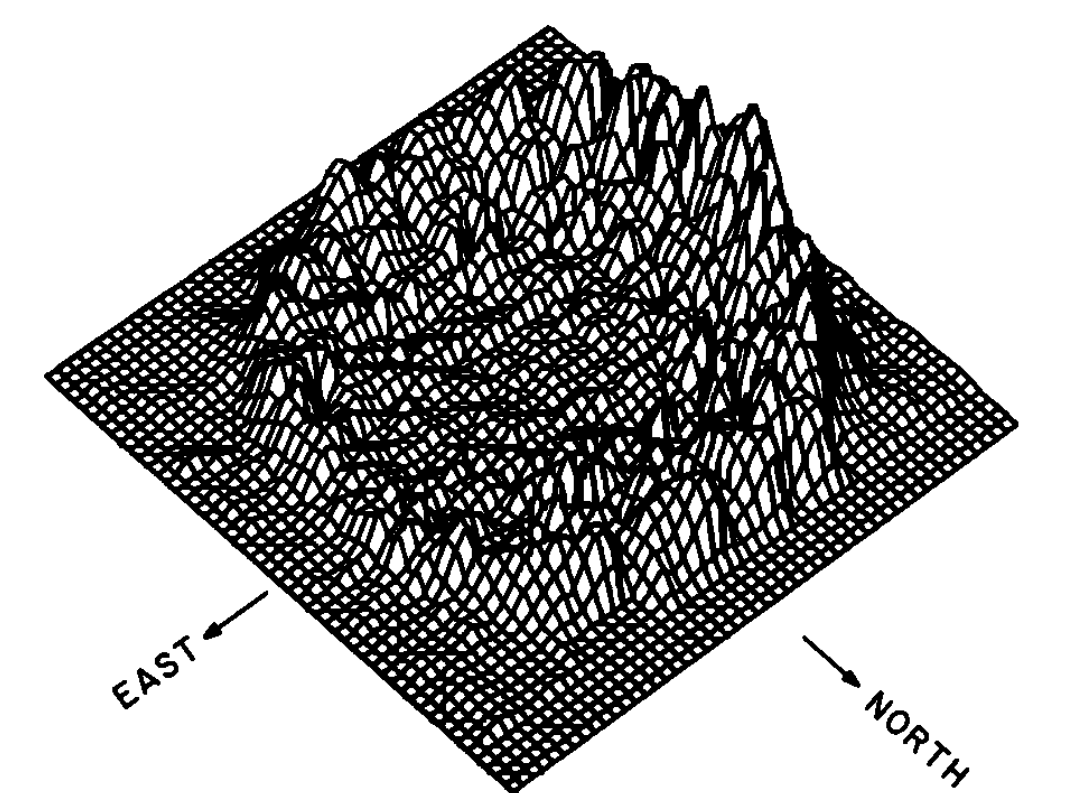
\includegraphics[width=0.48\textwidth]{content/literature_review/figures/sas2_map.png}
            }
        \hfill
         \subfloat[
            EGRET experiment \citep{Petry05}
         ]{
            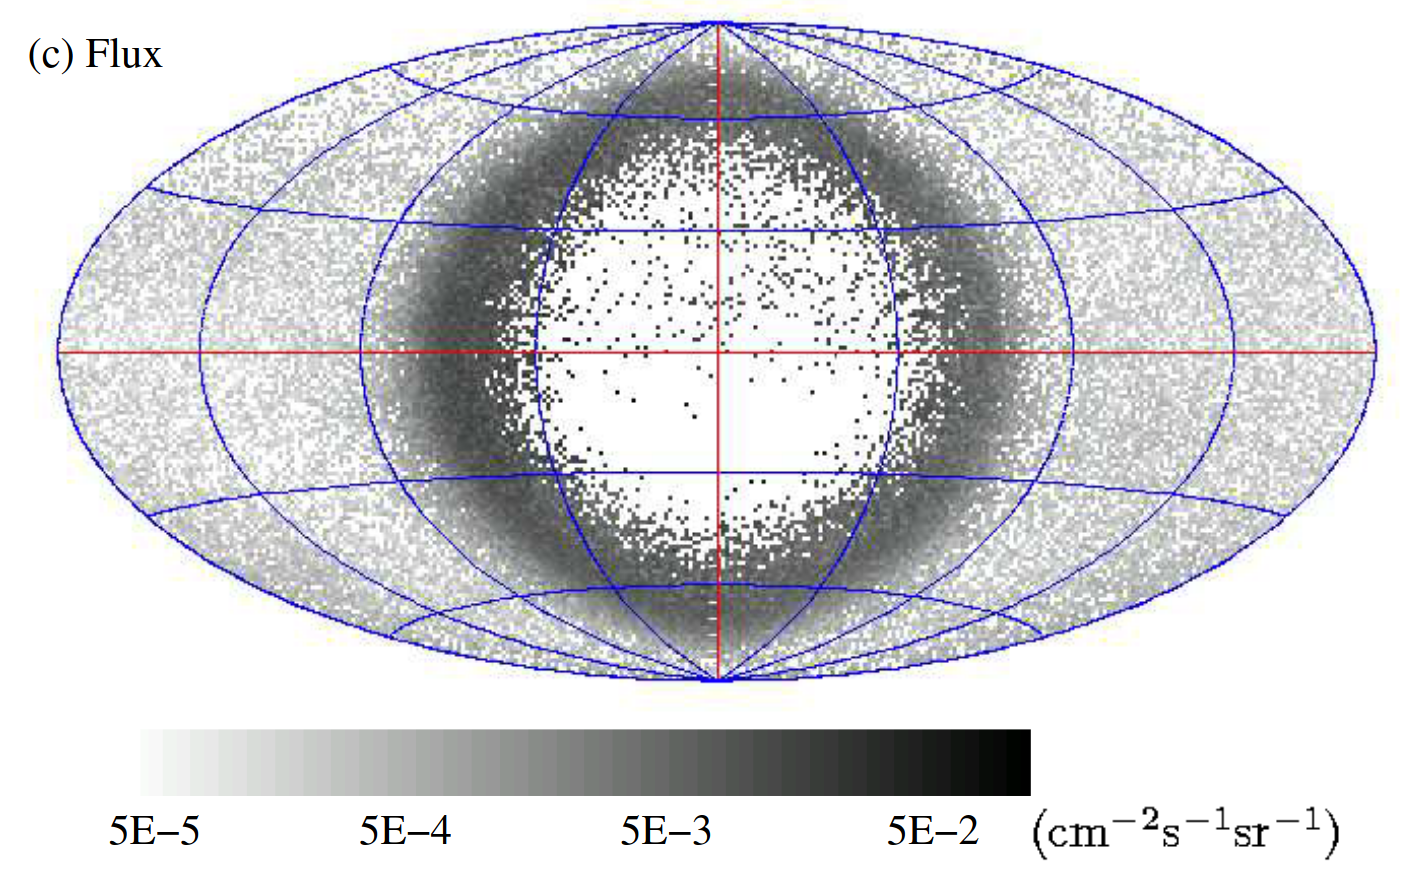
\includegraphics[width=0.48\textwidth]{content/literature_review/figures/egret_map.png}
        }
        \caption{
            The Earth's centered intensity plot from the satellite based observations
        }
       \label{fig:gamma_earth_second_wave}
\end{figure}

\cite{Morris84} showed the Earth's $\gamma$-ray intensity from different
line-of-sight atmospheric depth around the limb region
as plotted in Figure \ref{fig:emit_photon_vs_depth}, using data from \cite{Thompson81}.
% gamma from earth and moon \cite{Morris84}
% The previous details are full of so much experimental evidence.
% However, \cite{Morris84} put the weights on the assumption of 
% the bright region as seen as albedo in $\gamma$-ray came from the 
% interaction of proton and the atmospheric nuclei. The study
% shows the $\gamma$-rays intensity and the variation of air depth 
% by differing the zenith angle along limb region as plotted in 
% Figure \ref{fig:emit_photon_vs_depth} and \cite{Thompson81} data 
% has been exploited in the analysis.
This study computes the $\gamma$-ray spectrum from 
the bright region as seen from the Earth's and lunar limbs.
Figure \ref{fig:gamma_spectrum_earth_lunar} 
shows the spectrum from the theoretical calculation.
Figure \ref{fig:gamma_spectrum_earth_lunar}a
identifies the 2 bounds of the limb's region with an approximated air depth.
Solar activities can affact low-energy CR flux within the solar system.
This phenomenon can cause noticable change in the $\gamma$-ray
spectrum as demonstrated in Figure \ref{fig:gamma_spectrum_earth_lunar}b.

\begin{figure}[h!]
    \centering
    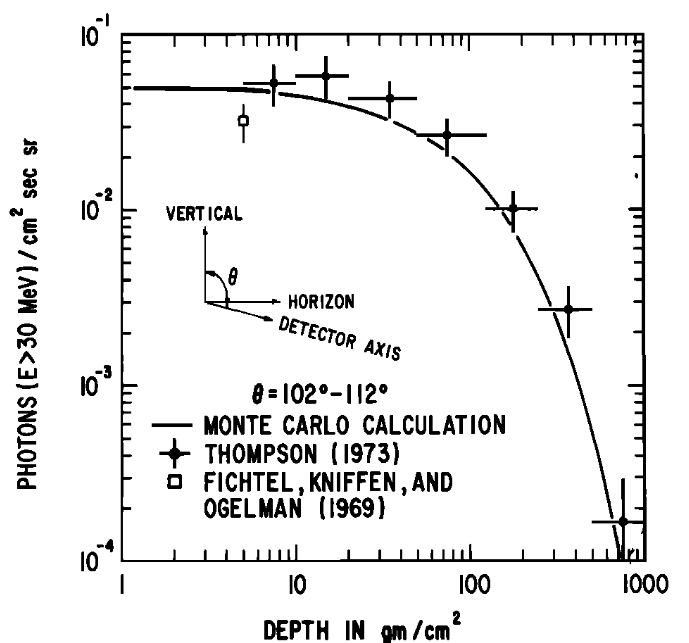
\includegraphics[width=0.6\textwidth]{content/literature_review/figures/morris_photon_vs_depth}
    \caption{
        Calculated $\gamma$-ray intensity
        at different atmospheric depth
        % with the variation of zenithal angle
        \citep{Morris84}
    }
    \label{fig:emit_photon_vs_depth}
\end{figure}

% Furthermore, this study computes the $\gamma$-ray spectrum from 
% the bright region as seen as albedo from the Earth's limb and 
% lunar albedo. The Figure \ref{fig:gamma_spectrum_earth_lunar} 
% shows the spectrum from the theoretical calculation. Figure \ref{fig:gamma_spectrum_earth_lunar}a
% identify the 2 bounds of the limb's region with an approximated air depth.
% Appealingly, another evidence of the solar activity could cause lower arrival CR particles since the propagating magnetic field 
% drag a charged particle towards outer space. The distinguishable
% spectrum from this phenomenon is demonstrated in
% Figure \ref{fig:gamma_spectrum_earth_lunar}b.


\begin{figure}[h!]
    \centering
        \subfloat[
            Earth's limb $\gamma$-ray spectrum
        ]{
            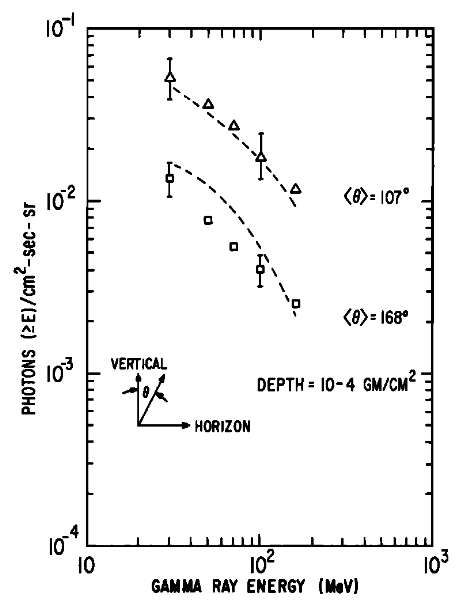
\includegraphics[width=0.48\textwidth]{content/literature_review/figures/morris_earth_spectrum.png}
            }
        \hfill
         \subfloat[
            Lunar's atmospheric $\gamma$-ray spectrum
         ]{
            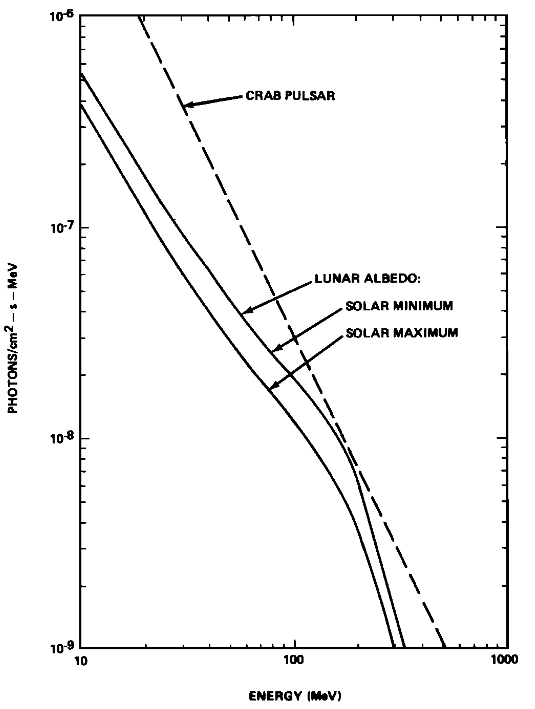
\includegraphics[width=0.48\textwidth]{content/literature_review/figures/morris_lunar_spectrum.png}
        }
        \caption{
            $\gamma$-ray spectrum from proton-nuclei interactions
            \citep{Morris84}
        }
       \label{fig:gamma_spectrum_earth_lunar}
\end{figure}


%% cr induced gamma-ray Fermi
\begin{figure}[h!]
    \centering
    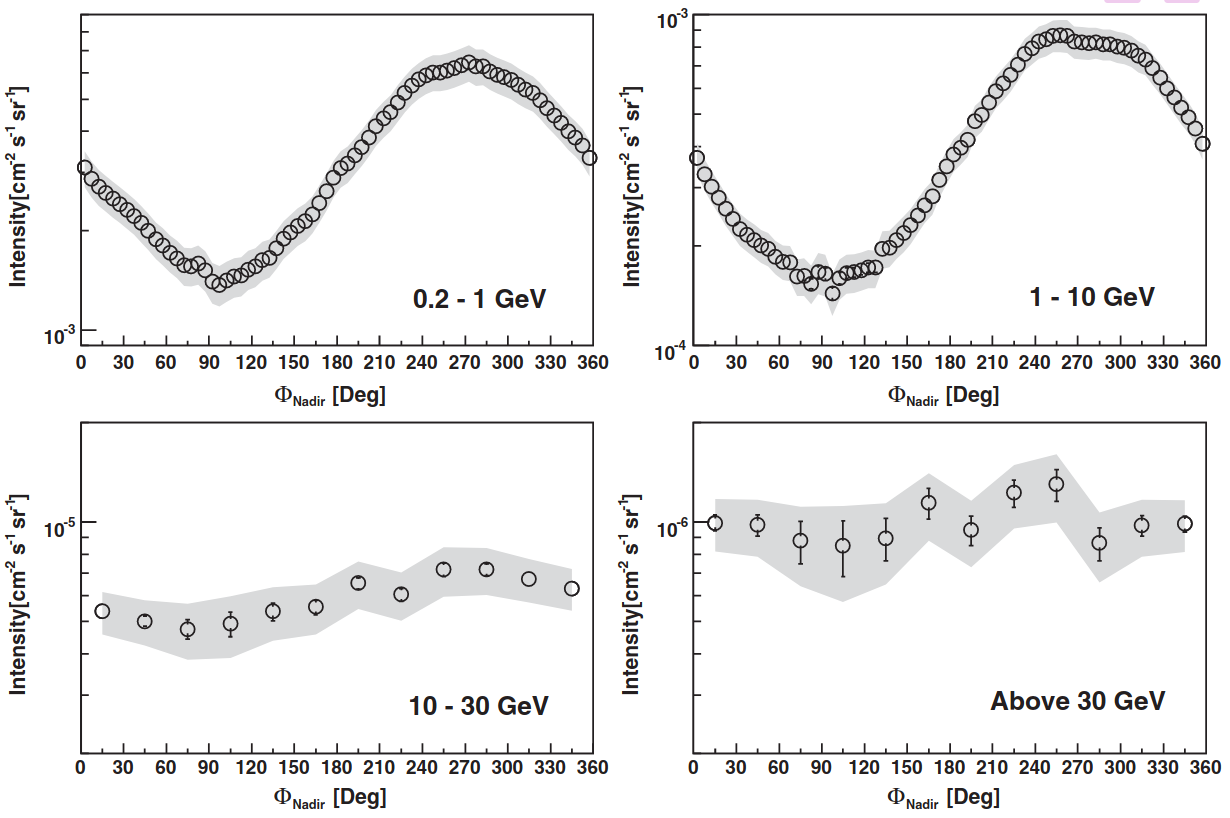
\includegraphics[width=0.9\textwidth]{content/literature_review/figures/fermi_eastwest.png}
    \caption{
        $\gamma$-rays intensity from limb emission in 4 energy ranges
        \citep{fermilat_gamma_induced}
    }
    \label{fig:fermi_eastwest}
\end{figure}

In 2009,
{\it Fermi} LAT released its first CR-induced Earth's
$\gamma$-ray emission analysis \cite{fermilat_gamma_induced}.
With technological improvements, the LAT is capable of detecting
$\gamma$ rays from ~100 MeV to near TeV with high angular resolution.
This study shows that the East-West effect is highly depends on the energy.
The effect is less prominent at high energy because CRs at
high rigidity are not deflected strongly by the Earth's
magnetic field as shown in Figure \ref{fig:fermi_eastwest}.
In addition, the latest study of Earth's $\gamma$-ray emission
from \cite{madlee2020} has clearly observed the 
effect in the spectrum at a few GeV scale.

% Ground-based detectors can detect atmospheric particles from
% CR-air interactions.
% A space-based detector can also inspect the East-West asymmetry
% effect from a low Earth orbit. In 2008, \textit{Fermi}-LAT was
% launched to observe $\gamma$ rays, and also electrons, and
% has clearly observed the East-West effect in the spectrum
% at a few GeV \citep{madlee2020}.


% Not so long after \textit{Fermi}-LAT was launched in the sky. In 2009,
% an early examination of the induced $\gamma$-ray emission was 
% observed by the most precise $\gamma$-ray detector
% \cite{fermilat_gamma_induced}. Since there 
% is a huge improvement in the technological side which makes LAT 
% capable of detecting high energy $\gamma$-ray from MeV up to TeV.
% Another discovery from this study was the East-West effect is highly 
% depends on the energy where it was converted from the incident energy of CR particles. The higher energy means the higher rigidity
% and it would reflect how hard the magnetic field could bend the trajectory.
% The intensity was divided into 4 energy ranges from a few GeV 
% to a higher GeV that could be considered as the relativistic scheme 
% where the kinetic energy is much higher than the mass as shown 
% in Figure \ref{fig:fermi_eastwest}.

% PAMELA proton&He cite:adriani2011pamela
% BESS: p&He cite: bess_experiment
% ams-02 proton cite:AMS02pr2015
% ams-02 helium cite:Heliumflux2015
The objective of this work is to indirectly measure the proton spectrum in 
the GeV range. The direct measurement in an early study of high-energy 
CR particles such as proton and helium was performed
by \cite{bess_experiment}.
More recently, PAMELA measured the proton and $\alpha$ spectra up
to ~TeV and reported an abrupt break in both spectra at a few
hundred GV with high significant level \citep{adriani2011pamela}.
% Another following experiment is \cite{adriani2011pamela}. Both of 
% them still lack the capability to detect such high energy on a scale of 
% a hundred GeV. Nevertheless, there is a clue about the breaking energy 
% in the proton spectrum with very low statistics and leaves room
% for further study.


% previous work (indirect measurement) : FermiEarth14
Although PAMELA claimed that the detection of the spectral break
was statistically significant, the break was close to its upper
energy limit and an independent confirmation would be important.
% Since there is just a clue from the previous direct observations.
An indirect measurement of CR proton spectrum has been performed in
energy between 90 GeV to 6 TeV by taking advantage of the brightness of
Earth's limb $\gamma$-ray emission from the collision of
incident CR protons \citep{FermiEarth14}.
This analysis used 5 years of Earth's $\gamma$-ray data along with
two proton-proton collision models to investigate the spectral
break of CR proton at a few hundred GV which PAMELA reported.
% The 5 years of $\gamma$-ray data have been exploited by investigating the incident proton spectrum via proton-proton collision model for finding whether CR protons have a breaking point of slope in the power 
% law spectrum. The study found that there is a breaking spectral index
% in the proton spectrum above 200 GeV 
% Nonetheless, Statistical analysis turns out that it is 1$\sigma$
% significant level.


One of the most recent space-based CR detectors, AMS-02, was installed
on the International Space Station in 2011 to study antimatter and
dark matter signals in CRs. 
% Back in 2011, one of the most efficient
% space-based CR detectors was launched by the carriage of the Endeavor
% space shuttle. The detector has been attached to the international space station (ISS).
% The main mission of AMS-02 is to search 
% antimatter, dark matter from measuring CRs.
AMS-02 can detect antimatter such as
positrons and antiprotons, and also
% position and antiproton. This detector is also able to detect
other heavyweight nuclei such as B, C, N, O, and Ne.
% like B, CNO, Ne, etc.
In 2015,
AMS-02 reported precision measurement of CR proton spectrum and
confirmed the spectral break at $\approx340$ GV at 99.9\%
confidence level \citep{AMS02pr2015}. 
% a proton spectrum has been directly
% reported and found the breaking at 340 GV \citep{AMS02pr2015}
% with very high statistics (confidence level 99.9\%).
The result from AMS-02 is consistent with other direct 
measurements from balloon-based and space-based experiments
% where the spectrum from various observations is plotted in 
as shown in Figure \ref{fig:ams02proton}.
In addition, the helium spectrum
was also measured and reported in \cite{Heliumflux2015}. 


\begin{figure}[h!]
    \centering
    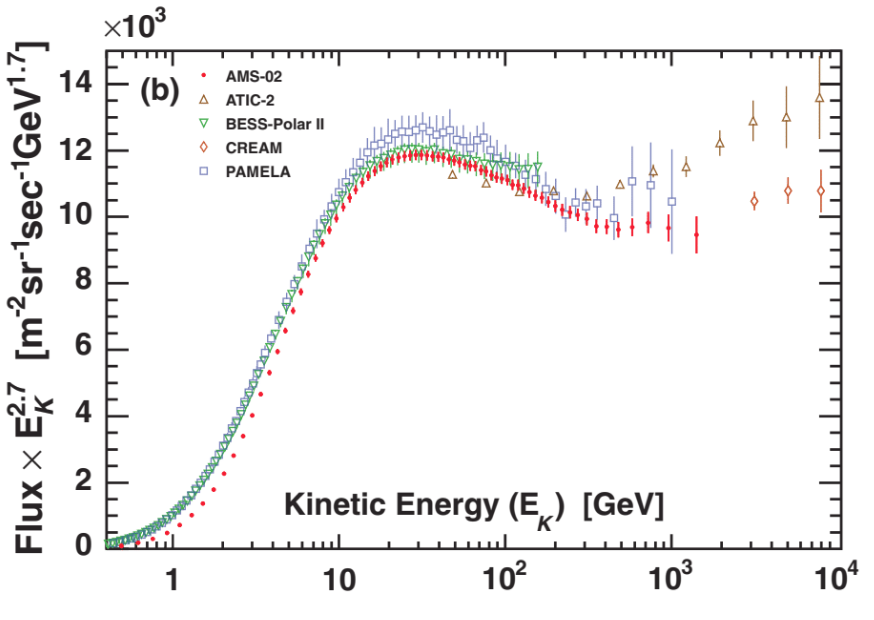
\includegraphics[width=0.75\textwidth]{content/literature_review/figures/direct_proton_measurement.png}
    \caption{
        CR proton spectrum from AMS-02 and earlier direct measurements
        \citep{AMS02pr2015}
    }
    \label{fig:ams02proton}
\end{figure}

% Turning back to the main objective of this work. The core concept 
% is to indirectly measure the proton CR spectrum 
According to the previous study \citep{FermiEarth14}, 
the detection of the CR proton spectral break at ~300 GV
is still at low significant level.
% low statistical significant potentially came from lack of the 
% dataset or the methodology from the consequence of indirect
% measurement.
In this work, a similar study will be performed with 
a larger data size from $\sim$ 9 years of observation.
% Hopefully, 
% the study could answer the first mentioned clue and put the weights
% on previous work.
Moreover, we improve the analysis
process by employing the heuristic optimization as well as using
high performance calculation of the exposure maps for faster
computational time of the Earth's $\gamma$-ray spectrum calculation. 